\clearpage
\lhead{COUNTRY_NAME Wikipedia}
\rhead{\thepage}

\vspace*{\fill}
\begin{center}
\Huge
COUNTRY_NAME Wikipedia
\end{center}
\vspace*{\fill}
\clearpage

\lhead{COUNTRY_NAME Wikipedia: Mining Vandalism}
\begin{figure}[t]
\centering\huge COUNTRY_NAME Wikipedia: Mining Vandalism
\end{figure}

\input{table-reverts-filtering-COUNTRY_CODE}
\begin{figure}[H]
\centering
\includegraphics[width=0.45\columnwidth]{revert-lengths-COUNTRY_CODE}
\caption{Number of full page reverts with a specific number of edits they revert and fitted exponential model in a log-log plot.}
\end{figure}

\clearpage

\lhead{COUNTRY_NAME Wikipedia: Geolocating Editors}
\begin{figure}[t]
\centering\huge COUNTRY_NAME Wikipedia: Geolocating Editors
\end{figure}
\begin{figure}[h]
\centering
\includegraphics{geolocation-decision-tree-COUNTRY_CODE}
\caption{Decision tree to decide whether to trust the available geolocation information for an edit (\protect
\includegraphics[scale=0.5]{../icon-accepted}), or not (\protect
\includegraphics[scale=0.5]{../icon-rejected}). The numbers denote the total edits and reverted edits for the COUNTRY_NAME Wikipedia that went through each branch.}
\vskip-1em
\end{figure}
\input{table-geolocation-overview-COUNTRY_CODE}
\begin{figure}[h]
\centering
\includegraphics[width=0.4\columnwidth]{full-agreement-num-iplocations-COUNTRY_CODE}
\caption{Number of total edits (white bars) and vandalism edits (gray bars) in millions from the yes-branch of Step (4) above over the number of GeoDBs considered.}
\end{figure}

\clearpage

\lhead{COUNTRY_NAME Wikipedia: Spatio-Temporal Analysis}
\begin{figure}[t]
\centering\huge COUNTRY_NAME Wikipedia: Spatio-Temporal Analysis\vskip-1em
\end{figure}
\input{table-wiki-country-count-revisions-by-COUNTRY_CODE}\vskip-1em
\input{table-wiki-country-count-vandalism-revisions-by-COUNTRY_CODE}\vskip-1em
\input{table-wiki-country-count-vandalism-commented-revisions-by-COUNTRY_CODE}
\noindent
The tables above show the number of certain kinds of edits from specific countries in all analyzed variants of Wikipedia. Countries are selected to have at least 100,000~vandalism edits in the COUNTRY_NAME Wikipedia, or that have COUNTRY_NAME as a major language (according to the English Wikipedia) and at least 1,000~vandalism edits. Countries are sorted by the number of all edits in the COUNTRY_NAME Wikipedia. The same countries are used in the hour-of-day plots.

Vandalism commented edits refers to edits that are---after filtering reverts---affected by a revert with a comment that signals that it is undoing vandalism (see Kittur et al. (2007b)). Note that this approach uses specific words to classify comments and is thus likely less effective in finding vandalism for other languages than English.

\begin{figure}[h]
\centering
\includegraphics[width=\textwidth]{world-absolute-COUNTRY_CODE}\\[3\baselineskip]
\includegraphics[width=\textwidth]{world-ratio-COUNTRY_CODE}
\caption{Number of edits (top) and ratio of vandalism to all edits (bottom) in the COUNTRY_NAME Wikipedia by country. Countries with less than 1,000~vandalism edits are not colored. The embedded small maps show (left) the vandalism ratio in the United States (without Alaska) by major time zone (from West to East: Pacific, Mountain, Central, and Eastern) with overlaid state borders and (right) Europe enlarged.}
\end{figure}

\begin{figure}[h]
\vskip-0.75em
\hrule
\centering
\begin{minipage}{.45\textwidth}%
\Large
COUNTRY_NAME Wikipedia\\[.3\baselineskip]
\normalsize
All plots show the ratio of vandalism to all edits per hour of day (left axis, solid lines), and for reference, the absolute number of edits (light gray) and vandalism edits (dark gray) per hour of day (right axis, dashed lines), both averaged over the COUNTRY_NAME Wikipedia's history. Ratios estimated from less than 1,000 vandalism edits are displayed with dotted lines.

The thin black line to the right is the vandalism ratio when detecting vandalism by comments of reverts (see Kittur et al. (2007b)). Note that this approach uses specific words to classify comments and is thus likely less effective in finding vandalism for other languages than English.
\end{minipage}\hfill%
\begin{minipage}{.45\textwidth}%
\includegraphics[width=\textwidth]{plot-by-hour-COUNTRY_CODE}%
\end{minipage}\\[\baselineskip]
\includegraphics[width=.45\textwidth]{plot-by-hour-and-weekday-COUNTRY_CODE}\hfill%
\includegraphics[width=.45\textwidth]{plot-by-hour-and-season-COUNTRY_CODE}\\
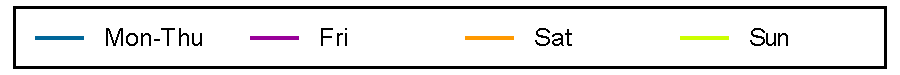
\includegraphics[width=.45\textwidth]{../weekday}\hfill%
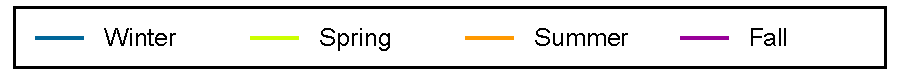
\includegraphics[width=.45\textwidth]{../season}
\hrule
\vskip-0.75em
\end{figure}

